%%%%%%%%%%%%%%%%%%%%%%%%%%%%%%%%%%%%%%%%%%%%%%%%%%%%%%%%%%%%%%%%%%%%%%%%%%%%%%%%
% \section{TOKIO Framework} \label{sec:methods}
\section{Instrumentation \& Data Sources} \label{sec:methods}
%%%%%%%%%%%%%%%%%%%%%%%%%%%%%%%%%%%%%%%%%%%%%%%%%%%%%%%%%%%%%%%%%%%%%%%%%%%%%%%%

%TOKIO is a framework that connects different sources of performance data that are already often collected by HPC facilities to present a holistic view of the I/O subsystem.
%TOKIO, schematically depicted in Figure \ref{fig:tokio-schematic}, integrates a combination of scalar and time-series data from sources available throughout the I/O subsystem and indexes them by time and job identifiers.
%This integration, detailed further in Section
%\ref{sec:data-integration}, enables systems staff to explore the
%climate of the I/O system over a time range of interest and relate this
%information to the weather of the I/O system for a particular job.
%%Furthermore, users can retrospectively examine the weather of the I/O system during their job and relate this information to the historic I/O system climate if TOKIO is deployed in an environment where users can access the required component-level monitoring data through a database or API.

% In the following sections we describe distinct components of the I/O subsystem that are critical to understanding both the I/O climate and I/O weather of a production system.
% Continuous instrumentation of each of these components should, therefore, be incorporated into TOKIO to enable the extraction of meaningful insight from the framework.
% We also provide pertinent details on the tools we have chosen to to instrument each of these components, preferring existing instrumentation solutions that are lightweight and unobtrusive enough to run full-time on production systems.
% The set of tools provided is not intended to be comprehensive or final--new data can be incorporated into TOKIO by defining mechanisms for accessing and indexing relevant data from a specific instrumentation source.

% \begin{figure}[t]
%    \centering
%    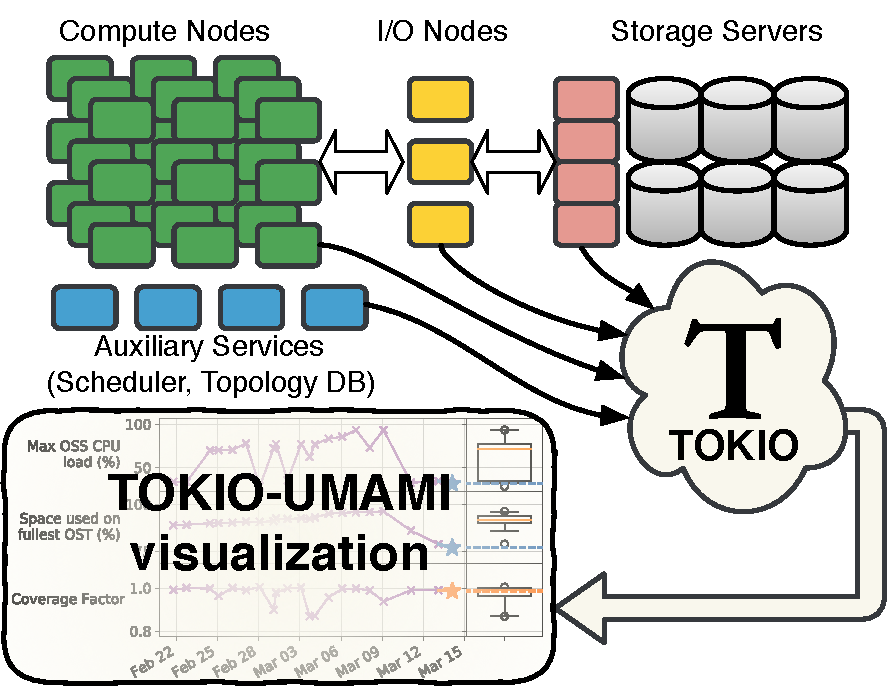
\includegraphics[width=.9\columnwidth]{figs/tokio-schematic.pdf}
%    \caption{Overview of the TOKIO framework.  Data is collected from sources
%    throughout the I/O subsystem, indexed and normalized, and then presented
%    through an interface that relates the I/O conditions of a specific job to the overall climate of the I/O subsystem.}
%    \label{fig:tokio-schematic}
%\vspace{-.2in}
%\end{figure}

\subsection{Application behavior} \label{sec:methods/darshan}

% Application behavior characterization describes the I/O pattern of a workload as expressed from the perspective of the application itself (i.e., before any system-level optimizations are applied).
To capture the I/O patterns and user-observable application performance in this study, we used the Darshan I/O characterization tool~\cite{carns200924} which transparently records statistics about an application's I/O behavior at runtime.
It imposes minimal overhead because it defers the reduction of these statistics until the application exits,
allowing it be deployed for all production applications on large-scale systems without perturbing performance.  Both systems used in this study link Darshan in compiled applications by default.
% Because it operates at the application level, Darshan is also highly portable across platforms.

\subsection{Storage system traffic} \label{sec:methods/storagesystraffic}

Storage system traffic monitoring provides insight into the aggregate system-wide I/O workload imposed on a target storage system.
On most modern-day HPC systems this is reflected in the aggregate bytes read and written, I/O operations processed, and other similar metrics collected at the parallel file system level.
This data can be collected in time-series format with minimal impact to application performance because it is gathered on the storage servers themselves without the involvement of the compute nodes.
For this study, we used two different file system-specific tools to collect this data.  These data were collected at five-second intervals as a trade-off between low performance impact and sufficient granularity to correlate performance with server activity~\cite{madireddy2017}.

\label{sec:methods/lmt}
\textbf{Lustre Monitoring Tool (LMT)} is a tool that aggregates Lustre-specific counters from /proc/fs/lustre on each Lustre object storage server (OSS) and metadata server (MDS) and presents them to external consumers via a MySQL database.
LMT provides time series data including bytes read and written, CPU load averages, and metadata operation rates.

\label{sec:methods/ggiostat}
\textbf{ggiostat} is a tool developed at ALCF to collect similar data from IBM Spectrum Scale (GPFS) file systems.
It includes a daemon that uses GPFS's \texttt{mmpmon} monitoring system to retrieve and store metrics from server and client clusters.
In this study, we examined bytes read and written, read and write request counts, and metadata operation counts.% which were collected on a per-cluster basis.

\subsection{Health monitoring} \label{sec:methods/health}

Health monitoring is critical to understanding the current fault status and capacity of the
storage system: what components are offline, failed-over, or another degraded state, and how much storage space remains on the available devices.
% lfs df
% lctl dl -t
To collect health-monitoring data on Lustre file systems, we record the fullness of each Lustre object storage target (OST) every fifteen minutes.
We also record the server to which each OST is mapped at this time, allowing us to identify OSTs that have failed over to a partner OSS and are degraded as a result.
% mmlsdisk
% mmdf
For GPFS, we record the fullness of each disk LUN and the failure status of each server when each job is submitted.
Recording the mapping between NSD servers and NSDs allows us to identify if a server has failed and a secondary server is handling its NSDs.
% In both GPFS and Lustre cases, we found that these time series data were sufficiently coarse-grained that storing these data in flat files indexed by date was sufficient.

\subsection{Job scheduling} \label{sec:methods/scheduling}

Job scheduling data can provide details on the mix of concurrent jobs that are running on the compute resources of a system to identify cases where I/O contention results from other competing workloads.
% Because job scheduling is most useful in the context of a particular job of interest, we represent this data as a single scalar value that represents the number of other jobs running concurrently with our job of interest.
Because job scheduling is most useful in the context of jobs which overlapped with our benchmark jobs of interest, we only considered a metric defined as the total number of other jobs running concurrently with our job of interest.

On the Edison system, this is accomplished by querying the Slurm job accounting database for all jobs with a start time before the job of interest's end time and an end time after the job of interest's start time.
Similarly, the job accounting data on Mira is uploaded by Cobalt into a database that can be accessed via a Python API called Ni.
The API allows pulling out a list of jobs for a given time range and running on a specific resource.

\subsection{Job Topology} \label{sec:methods/other}

% There are a number of other general and system-specific components that may
% affect I/O performance.  We anticipate that burst buffer metrics will play a
% critical role in emerging platforms, but we omit them in this study because
% our experimental platforms are not equipped with burst buffer hardware.
% Other examples of additional metrics that could be gathered include job layout and locality to I/O forwarding nodes, which
% can based on a job's node list and a topology map.
% In addition, network traffic on both compute and storage fabrics are often available through SNMP or vendor-specific monitoring tools.
% More comprehensive monitoring frameworks such as LDMS~\cite{7013000} can also serve as data repositories from which measurements can be drawn.
%
Job layouts on the Edison system were recorded for each job by combining queries to the Slurm accounting database, which maps jobs to node lists, and the Cray service database, which maps nodes to positions within the dragonfly network.
On Mira, jobs are always close-packed on its torus which results in identical layout for each job.
% The association between jobs and Lustre OSTs was also recorded in each job's Darshan log through the Darshan Lustre module.
% Similarly, job layout information on Mira was recorded in the Darshan logs
% through Darshan's Blue Gene/Q module~\cite{snyder2016modular}.  

% \subsection{Data integration} \label{sec:data-integration}

% The metrics outlined above are all integrated by the TOKIO framework by indexing the measurements from each data source by time and a unique job identifier.

% A given job's application behavior record is a logical starting point since it contains critical information including an estimate of I/O performance based on bytes moved and time spent in I/O.  It also contains job start time, end time, and its unique identifier, forming common indices with which storage system traffic, health monitoring, and job scheduling data can be aligned.

% In practice, our implementation of the TOKIO framework used in this study 
% To integrate the data from these disparate tools, we extracted summary metrics from each job's Darshan log and attached job scheduling data by joining on overlapping start and end timestamps.
% Health monitoring data was also joined to these data by identifying the last recorded health record before the job launched.
% Time series storage system traffic data such as that provided by LMT and ggiostat were reduced to scalar values (for example, as minimum, maximum, average bytes read per second) over the period each benchmark job was run.
% However, all of the time series data recorded between a job's start and end times are also retained as time-resolved slices which are then indexed using the job id.

% The resulting data structure is very concise and can be represented as a simple index of pointers to the raw files in which each I/O system component stores its measurements (e.g., Darshan logs or pyLMT HDF5 files).
% When transferring data between systems, all scalar measurements associated with a job can be serialized as a single row in a relational database or CSV-formatted file, and time series data can be encoded in a portable binary format such as HDF5.
% Because our implementation of TOKIO builds upon community software including Python and pandas, it can interact directly with a variety of data interfaces and
% natively supports indexing data located in relational databases (including MySQL, PostgreSQL, and SQLite) and serializing data to text and binary formats (including CSV, HDF5, and Excel spreadsheets).
% Ultimately, every system will have a different set of component-level monitoring tools in place, and TOKIO is designed to be sufficiently general to accept any scalar or time-series data available with only minor modification to its format or representation.

% In deploying the TOKIO framework and integrating data from multiple sources, we did encounter several noteworthy challenges.
% The most critical issue was ensuring that all components' clocks were synchronized to the same NTP servers to ensure that TOKIO's time-based indexing resulted in consistent data.
% Similarly, standardizing the frequency of time series data simplifies integration and data analysis; although we chose five-second sampling intervals for LMT and ggiostat, the health monitoring data was collected at very low frequency.
% To align such low-frequency data with scalar job data, we chose to treat health monitoring data as scalar data, and the sample that most recently preceded each job was associated that job.

%%%%%%%%%%%%%%%%%%%%%%%%%%%%%%%%%%%%%%%%%%%%%%%%%%%%%%%%%%%%%%%%%%%%%%%%%%%%%%%%
\section{Experimental Methods} \label{sec:platforms}
%%%%%%%%%%%%%%%%%%%%%%%%%%%%%%%%%%%%%%%%%%%%%%%%%%%%%%%%%%%%%%%%%%%%%%%%%%%%%%%%

%%% also used tablesgenerator.com to make this monstrosity
\begin{table*}[h]
\footnotesize
\centering
\begin{tabular}{|c|c|c|c|c|c|c|}
\hline
\textbf{\begin{tabular}[c]{@{}c@{}}System\\ (Center)\end{tabular}}                 & \textbf{Configuration}                                                                                         & \textbf{\begin{tabular}[c]{@{}c@{}}File System\\ (Type)\end{tabular}} & \textbf{\begin{tabular}[c]{@{}c@{}}\# Servers\\ (LUNs)\end{tabular}} & \textbf{\# I/O Nodes}                                                   & \textbf{\begin{tabular}[c]{@{}c@{}}Max\\ Capacity\end{tabular}} & \textbf{\begin{tabular}[c]{@{}c@{}}Peak\\ Performance\end{tabular}} \\ \hline
\multirow{3}{*}{\textbf{\begin{tabular}[c]{@{}c@{}}Edison\\
(NERSC)\end{tabular}}} & \multirow{3}{*}{\begin{tabular}[c]{@{}c@{}}Cray
XC-30\\5,586 CNs\end{tabular}} & scratch1 (Lustre)                                                     & 24 (24)                                                              & 9 (shared)                                                              & 2.2 PB                                                          & 48 GB/sec                                                           \\ \cline{3-7} 
                                                                                   &                                                                                                                & scratch2 (Lustre)                                                     & 24 (24)                                                              & 9 (shared)                                                              & 2.2 PB                                                          & 48 GB/sec                                                           \\ \cline{3-7} 
                                                                                   &                                                                                                                & scratch3 (Lustre)                                                     & 36 (36)                                                              & 13 (shared)                                                             & 3.3 PB                                                          & 72 GB/sec                                                           \\ \hline
\textbf{\begin{tabular}[c]{@{}c@{}}Mira\\ (ALCF)\end{tabular}}                     & \begin{tabular}[c]{@{}c@{}}IBM Blue Gene/Q\\ 49,152 CNs\end{tabular}    & mira-fs1 (GPFS)                                                       & 48 (336)                                                             & \begin{tabular}[c]{@{}c@{}}384 (dedicated)\\ 1 per 128 CNs\end{tabular} & 7.0 PB                                                          & 90 GB/sec                                                           \\ \hline
\end{tabular}
\caption{Test platforms for TOKIO and TOKIO Automated Benchmarking Collection (TOKIO-ABC)}
\label{tab:system-config}
\normalsize
\vspace{-.2in}
\end{table*}

To demonstrate the utility and generality of this holistic approach, we conducted a month-long experiment where we ran a series of I/O benchmarks every day on two distinct computing platforms:
Edison, a Cray XC-30 system at NERSC, and Mira, a Blue Gene/Q system at ALCF.
Over the course of this month-long period, we collected measurements from the data sources described in Section \ref{sec:methods} and used these data to
obtain a complete view of I/O during the time each benchmark job ran.
With this wide body of performance measurements and observed metrics, we performed statistical analysis to characterize the performance variability intrinsic to Edison and Mira (I/O climate) and contextualize the I/O behavior of specific jobs (I/O weather).
The analysis of these benchmark data reflect a total of 118 (Mira) and 1,014 (Edison) individual benchmark runs conducted over a period of 29 days (Mira) and 39 days (Edison).
%In this section, we detail the configuration of the benchmark suite used and the platforms on which they were run.

\subsection{I/O performance regression tests} \label{sec:methods/tests}

\noindent
%The instrumentation tools described in Section \ref{sec:methods} do not provide a fixed reference point on I/O behavior because
%the workload and state of the system evolve over time.
%To characterize the baseline behavior of Edison and Mira and define the climate of their I/O subsystems, we ran daily I/O performance regression tests based on both synthetic and application-derived workloads.
%We chose 
%a collection of benchmarks because performance is not well-represented
%by a single benchmark result; each storage system has its own strengths
%and weaknesses.  
%The collection of benchmarks is
%executed within a job script that can be scheduled nightly by a continuous
%integration system or cron job.  The script ensures that no more than
%one TOKIO-ABC instance is active at a time, and all benchmark results
%and Darshan logs are archived for analysis at the conclusion of the job.
%The initial set of benchmarks included in TOKIO-ABC are as follows:

We chose the size our benchmark runs to 
%The scale at which we ran each benchmark was governed by two goals:
a) saturate the storage system and
b) limit core-hour consumption sufficient for daily execution.
The specific benchmark configurations used are detailed in Table \ref{tab:bench-config}, and the four applications chosen are described as follows. 

The \textbf{Hardware Accelerated Cosmology Code (HACC)} framework~\cite{habib2012} is an N-body cosmology application
for simulating the the evolution of the Universe.
%from its early times to today and for understanding dark energy and dark matter.
We used the HACC-IO kernel which captures HACC's checkpoint I/O which generates
96 MiB/process 
%or 1.5 TiB total 
using POSIX file-per-process I/O.
%Each
%file is written in 10 large chunks, one chunk for each variable.

\textbf{Vector Particle-In-Cell (VPIC)} is a plasma physics application that simulates interactions among billions or trillions of particles \cite{Bowers2008}.
We used the VPIC-IO kernel which I/O operations of a magnetic reconnection simulation, where each MPI process writes $8 \times 2^{20}$ particles
%Each
%particle has eight properties (six floating point and two integer) and each
%property is a single dimension array. 
% The total number of particles depends on
%the number of MPI ranks used. 
to a single shared HDF5 file using the H5Part API \cite{H5Part}.
%and the execution of the I/O kernel includes
%creating and opening a file, writing data to the file, and closing the file.

The \textbf{BD-CATS} clustering system~\cite{Patwary2015} represents
a clustering analysis that is commonly performed on VPIC data.
We configured the BD-CATS I/O kernel to emulate the I/O workload of
a three-dimensional clustering that reads 75\% of the data
contained in the VPIC data file.

\textbf{IOR} is a widely used tool to characterize the performance of parallel file systems\cite{Yildiz2016,Xie2012,Lofstead2010,Uselton2010}.
For the purposes of this work, we applied IOR to determine each file system's performance variability under conditions where an application performs I/O using idealized parameters for each file system.

% abandon all hope ye who try to edit this stupid table by hand.  I used
% http://www.tablesgenerator.com to make it.
\begin{table}[h]
\footnotesize
\centering
\begin{tabular}{|c|c|c|c|c|c|c|c|}
\hline
 & \textbf{I/O Motif} & \textbf{Mira size} & \textbf{Edison size} \\
\hline
IOR & MPI-IO shared file & 1.0 TiB & 0.5 TiB\\
\hline
IOR & POSIX file per proc & 1.0 TiB & 2.0 TiB\\
\hline
HACC & POSIX file per proc & 1.5 TiB & 2.0 TiB \\
\hline
VPIC BD-CATS & HDF5 shared file & 1.0 TiB & 2.0 TiB\\
\hline
\end{tabular}
\caption{TOKIO-ABC benchmark configurations. All Mira benchmarks were
executed with 1,024 nodes and 16,384 MPI processes, while all Edison
benchmarks were executed with 128 nodes and 2,048 MPI processes.}
\label{tab:bench-config}
\normalsize
\vspace{-.4in}
\end{table}


\subsection{NERSC Edison} \label{sec:platforms/edison}

Edison is a Cray XC-30 system deployed at the National Energy Research Scientific Computing Center (NERSC) whose architecture is described in Table \ref{tab:system-config}.
Its scratch1 and scratch2 file systems are identically configured, and users are evenly distributed across both such that the two file systems should have similar levels of I/O traffic.
However, access to Edison's scratch3 file system is only granted to users who require high parallel bandwidth, and therefore the scratch3 file system should reflect larger, more coherent I/O traffic.

The Edison architecture routes I/O traffic from the Cray Aries high-speed network to the FDR InfiniBand-based SAN fabric through LNET I/O nodes.
Routing is configured such that each LNET I/O node handles traffic for only one of the three Edison file systems.
%As a result of this design and the use of Lustre fine-grained routing, all jobs on Edison that utilize one file system share the same set of I/O nodes.
This ensures that each file system's traffic is isolated as it transits I/O nodes and also allows every Edison job to use the maximum number of I/O nodes.

The benchmark configurations for the Edison file systems are described in Table \ref{tab:bench-config}.
In all cases, data was striped over all of the OSTs in the file system, and the input parameters listed in Table \ref{tab:bench-config} were chosen specifically to saturate each file system's bandwidth.
As such, the IOR benchmark configurations demonstrated peak performance at 90\% of the theoretical peaks listed in Table \ref{tab:system-config}.

\subsection{ALCF Mira} \label{sec:platforms/mira}

Mira is an IBM Blue Gene/Q system deployed at the Argonne Leadership Computing Facility (ALCF) whose architecture is detailed in Table \ref{tab:system-config}.
In addition to the servers and LUNs listed, six of the network shared disk (NSD) servers also have an SSD-based LUN on which metadata is stored.
% Mira also has has another primary file system not used in this study, mira-fs0, which shares the same InfiniBand SAN fabric as mira-fs1.
% Although these file systems have independent NSD servers and devices, I/O can still contend for resources on this storage network.

Unlike Edison, Mira's I/O architecture has fixed-size partitions of compute nodes connected to each I/O forwarding node, 
meaning that storage bandwidth available through I/O nodes scales linearly with the size of the compute job.
% Running daily I/O benchmarks that span a large portion of Mira's compute nodes is impractical due to the lengthy queue times of capability jobs and the disruption this would have to job scheduling.
%Therefore the job size used on Mira, 1,024 Mira compute nodes (a single rack), was based upon the availability of compute resources rather than the saturation of I/O subsystem.
To minimize system system disruption and maximize throughput of our daily benchmarks, we opted to run every benchmark using 1,024 compute nodes which 
corresponds to eight I/O nodes and an aggregate peak bandwidth of ~25 GB/sec.
In practice, the IOR configuration for Mira listed in Table \ref{tab:bench-config} was able to achieve 80\% of this peak performance of this I/O node allocation.
